\chapter{Simulation model}
\label{chap:simulation_model}

\section{General structure}

\subsection{Classes of the model}
The model is developed in Python and consists of two classes (see fig. \ref{uml}) : the HydropowerPlant class, which represents a run-of-the-river power plant and the Modelchain class which represents the simulation of one plant. The attributes and methods of each class are detailled in table \ref{att_meth}. \newline
A Modelchain object takes a HydropowerPlant object as input, as well as runoff time series. If attributes from the HydropowerPlant object are missing, the Modelchain object calculates them during initialization, through the extrapolation process presented in subsection \ref{sub:extrapolation}. The implementation of this process is detailed in subsections \ref{sub:check_feas} to \ref{sub:get_type}.
\begin{figure}[H]
\center
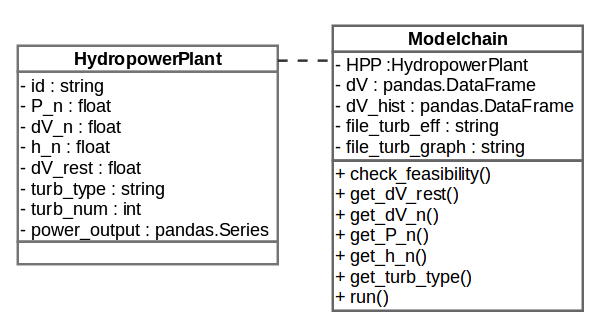
\includegraphics[width=12cm]{uml.png}
\caption{Classes of the hydropower model}
\label{uml}
\end{figure}

\begin{table}
\footnotesize
 \caption{Attributes and methods of the classes}
 \centering
 \label{att_meth}
 \begin{tabular}{|l|l|l|p{6cm}|}
  \cline{2-4}
  \multicolumn{1}{c|}{}&\multicolumn{3}{c|}{\textbf{class HydropowerPlant}}\\ \hline
  \multirow{8}{*}{\rotatebox[origin=c]{90}{\textbf{Attributes}}}&id&string&Identification of the plant\\
  &P{\_}n&float&Nominal power of the plant in \unit{W}\\
  &dV{\_}n&float&Nominal inflow of the plant in \unit{m\textsuperscript{3}\textperiodcentered s\textsuperscript{-1}}\\
  &h{\_}n&float&Nominal head of water in \unit{m}\\
  &dV{\_}rest&float&Residual water flow in \unit{m\textsuperscript{3}\textperiodcentered s\textsuperscript{-1}}\\
  &turb{\_}type&string&Type of turbine(s)\\
  &turb{\_}num&int&Number of turbines. Default : 1\\
  &power{\_}output&pandas.Series&Power output in \unit{W}\\
  \hline
  \multicolumn{4}{c}{}\\
  \cline{2-4}
  \multicolumn{1}{c|}{}&\multicolumn{3}{c|}{\textbf{class Modelchain}}\\ \hline
  \multirow{5}{*}[-1cm]{\rotatebox[origin=c]{90}{\textbf{Attributes}}}&HPP&HydropowerPlant&Plant to simulate\\
  &dV&pandas.DataFrame&Runoff time series in \unit{m\textsuperscript{3}\textperiodcentered s\textsuperscript{-1}} with DateTime index over the period to simulate\\
  &dV{\_}hist&pandas.DataFrame&Runoff time series in \unit{m\textsuperscript{3}\textperiodcentered s\textsuperscript{-1}} with DateTime index over several past years\\
  &file{\_}turb{\_}eff&string&File containing parameters about turbine efficiencies\\
  &file{\_}turb{\_}graph&string&File containing the characteristic diagrams\\
  \hline
  \multirow{7}[5]{*}{\rotatebox[origin=c]{90}{\textbf{Methods}}}&check{\_}feasibility()&boolean&Checks if input data is sufficient \\
  &get{\_}dV{\_}rest()&float&Calculates residual runoff in \unit{m\textsuperscript{3}\textperiodcentered s\textsuperscript{-1}}\\
  &get{\_}dV{\_}n()&float&Calculates nominal runoff in \unit{m\textsuperscript{3}\textperiodcentered s\textsuperscript{-1}}\\
  &get{\_}P{\_}n()&float&Calculates nominal power in \unit{W}\\
  &get{\_}h{\_}n()&float&Calculates nominal head in \unit{m}\\
  &get{\_}turb{\_}type()&string&Finds type of turbine\\
  &run()&void&Calculates HPP.power{\_}output in \unit{W}\\
  \hline
 \end{tabular}
\end{table}

\subsection{Inputs and outputs}

The HydropowerPlant class has one compulsory parameter (id) and six optional parameters (P{\_}n, dV{\_}n, h{\_}n, dV{\_}rest, turb{\_}type, turb{\_}num). The number of turbines (turb{\_}num) is by default set to one when not filled in and the other optional parameters are extrapolated in the Modelchain class. \newline 
The Modelchain class takes pandas DataFrames as input for runoff. They can be read from csv files or extracted from a database, as presented in sections \ref{sub:ex_with_csv} and \ref{sub:ex_with_oedb}. These DataFrames require a DateTime index and a column named 'dV' containing runoff values. In order to correctly extrapolate the nominal water flow and the residual water flow from the historic values, DataFrame 'dV{\_}hist' has to cover many years (10 to 25 according to \cite{pacer} and \cite{cetmef}). Moreover, the time series should preferably be of whole years to avoid errors due to seasonal changes. \newline
The output power in \unit{W} is stored in the power{\_}output attribute of the HydropowerPlant object, as a pandas Series with the same DateTime index as the input 'dV' DataFrame.

\section{Implementation details}

\subsection{Initialization of Modelchain class}

When a Modelchain object is created. an initialization process takes place to check the integrity of the input and if needs be extrapolate the missing input data. The initialization process is presented in figure \ref{init} and the different methods are detailed in the following sections.

\begin{figure}[H]
\center
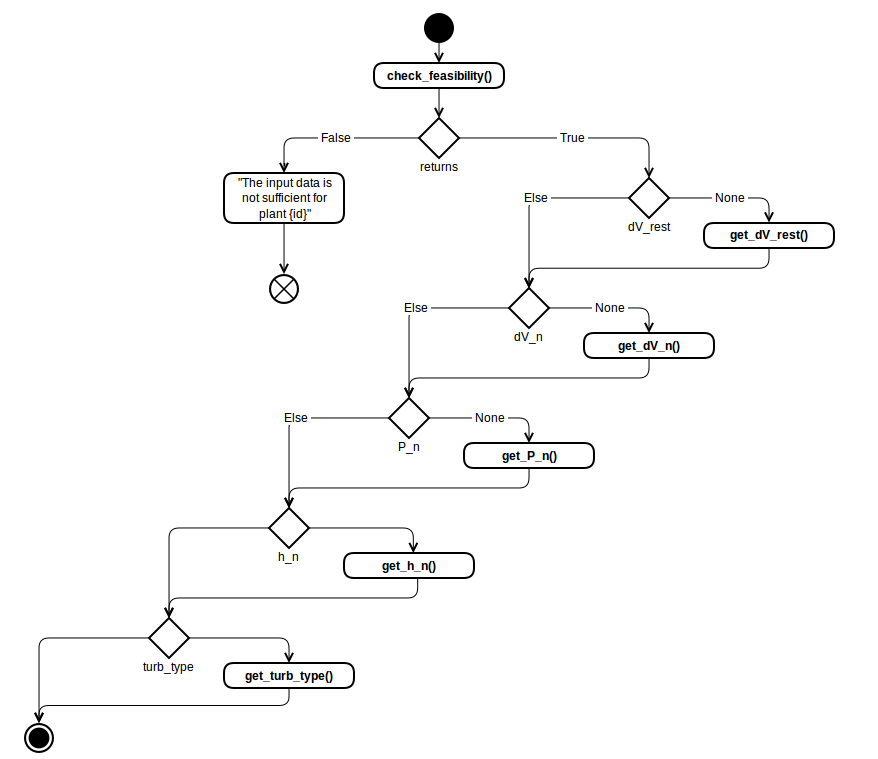
\includegraphics[width=15cm]{init.png}
\caption{Initialization of Modelchain class}
\label{init}
\end{figure}

\subsection{Method check{\_}feasibility()}
\label{sub:check_feas}

When a Modelchain object is initialized, the missing parameters of the HydropowerPlant object are extrapolated from the known parameters and the runoff history. For the extrapolation to be possible, enough parameters have to be filled in. With two parameters among  P{\_}n, dV{\_}n and h{\_}n can the third be calculated using the power equation in nominal operation (eq. \ref{eq_nom}) with nominal efficiencies of the generator and the turbine approximated to respectively 95\% and 90\%. If the runoff history is filled in, it can be use to extrapolate the nominal and residual water flows. If it is not filled in, the residual water flow can be set to 0 as it is very small part of the actual water flow. The type of turbine is then extrapolated from the nominal head and water flow.
\begin{equation}
\label{eq_nom} 
 P_\mathrm{n} = \rho_\mathrm{water} \cdot g \cdot \dot{V}_\mathrm{n} \cdot h_\mathrm{n} \cdot \eta_\mathrm{turbine, n} \cdot \eta_\mathrm{generator, n}
\end{equation}

Therefore, the first step of the initialization is to check the feasibility of the simulation. This is done with a logical test on the presence of inputs. The logical expression, obtained by filling in a Karnaugh map (see fig. \ref{karnaugh}), is given in equation \ref{eq_feas}.

\begin{equation}
\label{eq_feas} 
 Feasibility = (h_\mathrm{n} \land P_\mathrm{n}) \lor ((h_\mathrm{n} \lor P_\mathrm{n}) \land (\dot{V}_\mathrm{hist} \lor \dot{V}_\mathrm{n}))
\end{equation}

\begin{figure}[H]
\caption{Karnaugh map of simulation feasibility depending on inputs}
\center
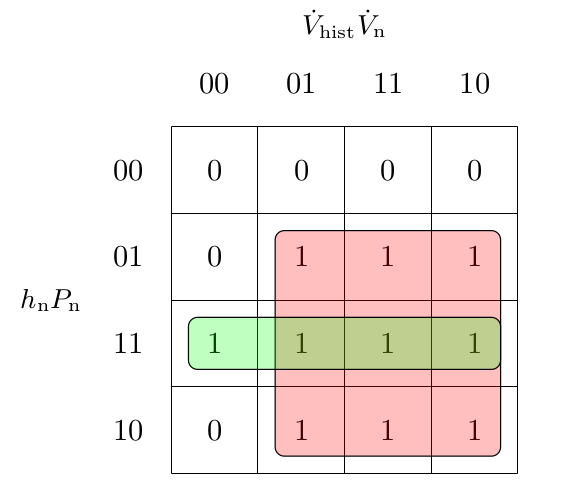
\includegraphics[width=8cm]{karnaugh.png}
\label{karnaugh}
\end{figure}

\subsection{Method get{\_}dV{\_}rest()}

The approach chosen to calculate the residual water flow is given in section \ref{sub:extrapolation}. It is implemented in the model within the get{\_}dV{\_}rest() method of the Modelchain class, called during initialization.\newline If no runoff history has been specified, the residual water flow is set to zero. Otherwise, the ten most recent years of the runoff history are aggregated in a mean flow duration curve from which \.{V}\textsubscript{347} is extracted as the water flow attained or exceeded 347 days a year. The residual water flow \.{V}\textsubscript{rest} is then calculated following table \ref{res_wat} page \pageref{res_wat}. \newline
The python script of this method is given in appendix \ref{app:get_dV_rest}.

\subsection{Methods get{\_}dV{\_}n(), get{\_}h{\_}n() and get{\_}P{\_}n()}

If the nominal head and nominal power are given, the nominal water flow is calculated using equation \ref{eq_dV_n} with $\eta_\mathrm{turbine, n} = \unit[90]{\%}$ and $\eta_\mathrm{generator, n} = \unit[95]{\%}$.\newline

\begin{equation}
\label{eq_dV_n} 
 \dot{V}_\mathrm{n}=\frac{ P_\mathrm{n}}{\rho_\mathrm{water} \cdot g  \cdot h_\mathrm{n} \cdot \eta_\mathrm{turbine, n} \cdot \eta_\mathrm{generator, n}}
\end{equation}

If the nominal head or nominal water flow are missing, a history of water flows has to be specified for the simulation to be possible, and the nominal water flow is extrapolated from this history. The approach chosen to calculate the nominal water flow is given in section \ref{sub:extrapolation}. It is implemented in the model within the get{\_}dV{\_}rest() method of the Modelchain class, called during initialization.\newline

\subsection{Method get{\_}turb{\_}type()}
\label{sub:get_type}
\subsection{Calculate power output}
\section{Use examples}
\subsection{With csv files}
\label{sub:ex_with_csv}
\subsection{With the OpenEnergy Database}
\label{sub:ex_with_oedb}